\section{实验结果}
\subsection{在 UNIX V6++ 中编译链接运行一个 C 语言程序并调试}
如图\ref{newFile}-\ref{exec}所示,首先,我在programs文件夹下添加了showStack.c文件,
然后在命令行中运行make all命令,显示build success;接着,在远程桌面中运行make qemu,并在bin文件夹下调用showStack程序,
输出result=3,符合预期;最后,我在main1函数的result=sum(a,b)处打上断点,并在远程桌面中执行make qemug,同时在vscode切换调试对象为showStack程序,并启动调试。
断点命中后,右键CALL STACK栏中的main1()项,并点击Open Disassembly View,可以在打开的汇编代码界面中查看
命中的断点位置对应的汇编代码。此时,我还在debug console中通过执行-exec x /20xw 0x7fffc0来视察0x7fffc0处的内存空间。
\begin{figure}[!htbp]
    \centering
    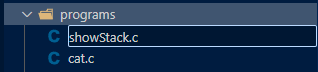
\includegraphics[scale=1]{figures/newFile.png}
    \caption{加入新的c语言文件}\label{newFile}
\end{figure}

\begin{figure}[!htbp]
    \centering
    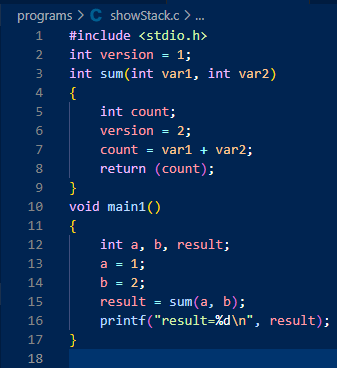
\includegraphics[scale=1]{figures/newCode.png}
    \caption{加入新的c语言文件}\label{newCode}
\end{figure}

\begin{figure}[!htbp]
    \centering
    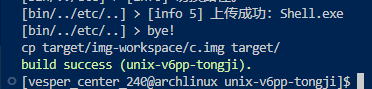
\includegraphics[scale=1]{figures/buildSuccess.png}
    \caption{编译成功}\label{buildSuccess}
\end{figure}

\begin{figure}[!htbp]
    \centering
    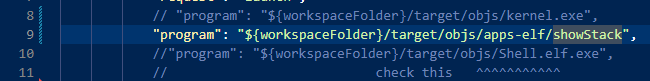
\includegraphics[width=\textwidth]{figures/switch.png}
    \caption{切换调试目标}\label{switch}
\end{figure}

\begin{figure}[!htbp]
    \centering
    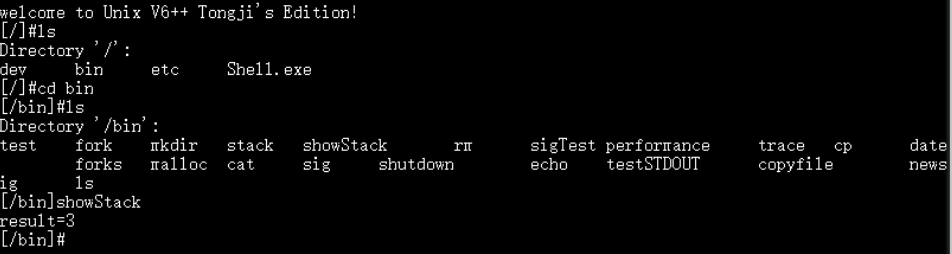
\includegraphics[width=\textwidth]{figures/showStack.png}
    \caption{调试showStack程序}\label{showStack}
\end{figure}

\begin{figure}[!htbp]
    \centering
    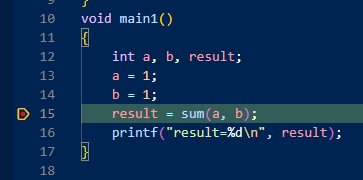
\includegraphics[scale=1]{figures/breakpoint.png}
    \caption{触发断点}\label{breakpoint}
\end{figure}

\begin{figure}[!htbp]
    \centering
    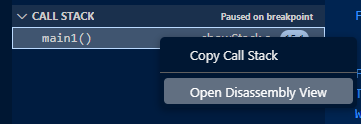
\includegraphics[scale=1]{figures/disassembly.png}
    \caption{查看汇编代码}\label{disassembly}
\end{figure}

\begin{figure}[!htbp]
    \centering
    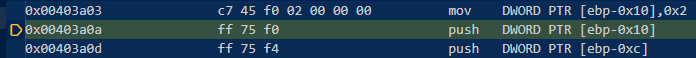
\includegraphics[width=\textwidth]{figures/discode.png}
    \caption{汇编代码界面}\label{discode}
\end{figure}

\begin{figure}[!htbp]
    \centering
    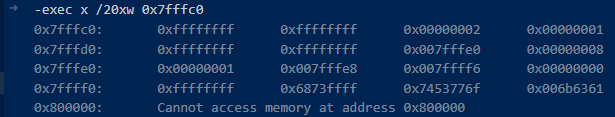
\includegraphics[scale=1]{figures/exec.png}
    \caption{视察内存单元值}\label{exec}
\end{figure}
\clearpage
\subsection{观察 main1 函数堆栈的变化}
如图\ref{entermainBFPushEBP}所示,执行push ebp后,ebp值0x007ffe0入栈。

\begin{figure}[!h]
    \centering
    \includegraphics[scale=1]{figures/entermainBFPushEBP.png}
    \caption{执行push ebp前后用户栈的状况}\label{entermainBFPushEBP}
\end{figure}

如图\ref{BFValue}所示,给main1中的局部变量a,b分别赋值1,2后,可以看到,用户栈中的两个相邻内存单元分别被赋值1,2。

\begin{figure}[!htbp]
    \centering
    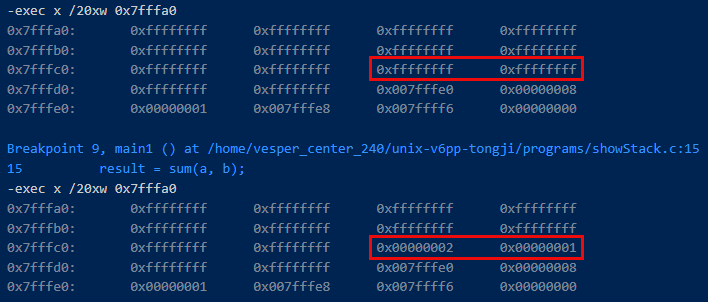
\includegraphics[width=\textwidth]{figures/BFValue.png}
    \caption{给局部变量a,b赋值前后用户栈的状况}\label{BFValue}
\end{figure}

如图\ref{beforeCall}所示,执行call之前,实参var2,var1的值被依次压入栈中。

\begin{figure}[!htbp]
    \centering
    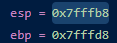
\includegraphics[scale=1]{figures/regBeforeCall.png}
    \caption{执行call之前的esp与ebp中的值}\label{regBeforeCall}
\end{figure}

\begin{figure}[!htbp]
    \centering
    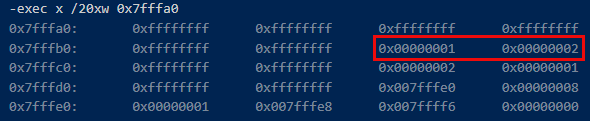
\includegraphics[scale=1]{figures/beforeCall.png}
    \caption{执行call之前的用户栈的状况}\label{beforeCall}
\end{figure}


\subsection{观察 sum 函数堆栈的变化}
\begin{minted}{asm}
push ebp                       ; 旧ebp入栈
mov ebp, esp                   ; 更新栈帧
sub esp, 0x10                  ; 为局部变量预留空间
mov DWORD PTR ds:0x4042f4, 0x2 ; 为全局变量version赋值
mov edx, DWORD PTR [ebp+0x8]   ; 取var2的值
mov eax, DWORD PTR [ebp+0xc]   ; 取var1的值
add eax, edx                   ; 相加
mov DWORD PTR [ebp-0x4], eax   ; 将结果赋值给局部变量
mov eax, DWORD PTR [ebp-0x4]   ; 将待返回值存储至eax中
leave 
ret 
\end{minted}

\begin{figure}[!htbp]
    \centering
    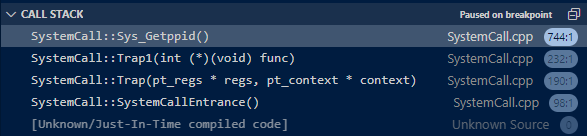
\includegraphics[scale=1]{figures/stack.pdf}
    \caption{执行leave前用户栈的情况}\label{stack}
\end{figure}

如图\ref{afterCall}所示,执行call之后,返回地址压入栈中。

\begin{figure}[!htbp]
    \centering
    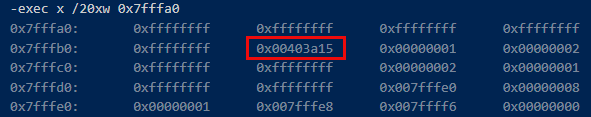
\includegraphics[scale=1]{figures/afterCall.png}
    \caption{执行call后用户栈的状况}\label{afterCall}
\end{figure}

如图\ref{afterPush}所示,执行push ebp之后,main1的栈帧对应的ebp压入栈中。

\begin{figure}[!htbp]
    \centering
    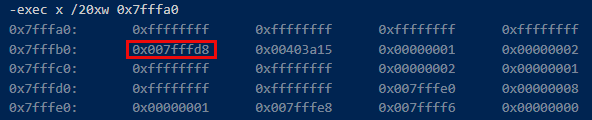
\includegraphics[scale=1]{figures/afterPush.png}
    \caption{执行push ebp前后用户栈的状况}\label{afterPush}
\end{figure}

如图\ref{afterAdd}所示,执行count=var1+var2之后,ebp-0x4处被赋值3。


\begin{figure}[!htbp]
    \centering
    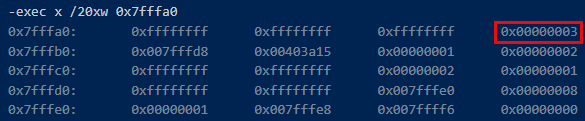
\includegraphics[scale=1]{figures/afterAdd.png}
    \caption{执行count=var1+var2后用户栈的状况}\label{afterAdd}
\end{figure}

如图\ref{afterLeave}所示,执行leave后,esp指向返回地址,ebp指向main1栈帧对应的ebp。

\begin{figure}[!htbp]
    \centering
    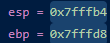
\includegraphics[scale=1]{figures/afterLeave.png}
    \caption{执行leave后esp与ebp的值}\label{afterLeave}
\end{figure}

如图\ref{afterRet}所示,执行ret后,返回地址出栈,并赋值给eip。

\begin{figure}[!htbp]
    \centering
    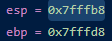
\includegraphics[scale=1]{figures/afterRet.png}
    \caption{执行ret后esp与ebp的值}\label{afterRet}
\end{figure}

\begin{figure}[!htbp]
    \centering
    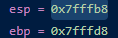
\includegraphics[scale=1]{figures/beforeAddESP.png}
    \caption{执行add esp,0x8之前的esp与ebp的值}\label{beforeAddESP}
\end{figure}

如图\ref{stack}所示,\textcolor{red}{之所以此时需要执行add esp,0x8,是为了舍弃之前为了调用sum函数而压入栈的两个实参}。

\textcolor{red}{如图\ref{beforemain}-\ref{afterexec}所示,可以看到各个关键时刻ds:0x4042f4处的值。显然,该处是Data段,存放着
全局变量version。该处一开始为不可知值,在刚刚进入main1函数时,便已被置1。同时,mov DWORD PTR ds:0x4042f4,0x2后0x7fffc0对应的c语言语句是
version=2。}

\begin{figure}[!htbp]
    \centering
    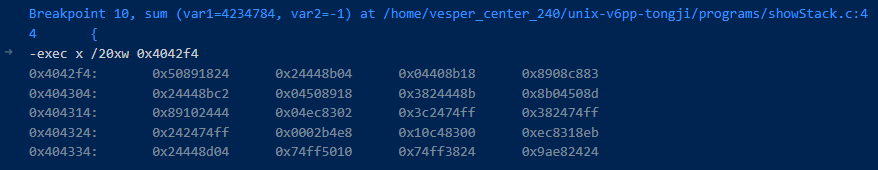
\includegraphics[width=\textwidth]{figures/beforemain.png}
    \caption{进入main1函数前0x7fffc0处内存的状况}\label{beforemain}
\end{figure}
\begin{figure}[!htbp]
    \centering
    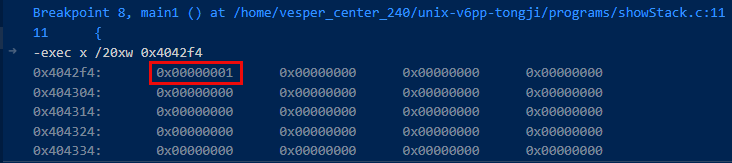
\includegraphics[width=\textwidth]{figures/aftermain.png}
    \caption{进入main1函数后0x7fffc0处内存的状况}\label{aftermain}
\end{figure}
\begin{figure}[!htbp]
    \centering
    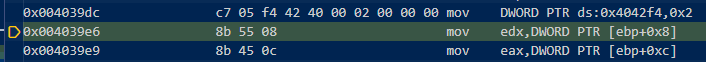
\includegraphics[width=\textwidth]{figures/exec02.png}
    \caption{执行mov DWORD PTR ds:0x4042f4,0x2后}\label{exec02}
\end{figure}
\begin{figure}[!htbp]
    \centering
    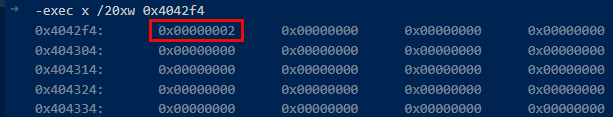
\includegraphics[width=\textwidth]{figures/afterexec.png}
    \caption{执行mov DWORD PTR ds:0x4042f4,0x2后0x7fffc0处内存的状况}\label{afterexec}
\end{figure}


